\documentclass[11pt,a4paper]{article}
\usepackage[utf8]{inputenc}
\usepackage[spanish,es-tabla]{babel}
\usepackage{amsmath}
\usepackage{amsfonts}
\usepackage{amssymb}
\usepackage{graphicx}
\usepackage{float}
\usepackage{cite}

\usepackage{xcolor,colortbl}

\newcommand{\mc}[2]{\multicolumn{#1}{c}{#2}}
\definecolor{Gray}{gray}{0.85}
\definecolor{LightCyan}{rgb}{0.88,1,1}
\definecolor{DayliGreen}{rgb}{0.8, 0.85, 0.84}
\definecolor{LightGreen}{rgb}{0, 1, 0.72}

\newcolumntype{a}{>{\columncolor{white}}c}
\newcolumntype{b}{>{\columncolor{white}}c}


\usepackage{hyperref}

\usepackage{vmargin}

\setpapersize{A4}
\setmargins{2.5cm}              % margen izquierdo
{1.5cm}                         % margen superior
{16.5cm}                        % anchura del texto
{23.42cm}                       % altura del texto
{10pt}                          % altura de los encabezados
{1cm}                           % espacio entre el texto y los encabezados
{0pt}                           % altura del pie de página
{2cm}                           % espacio entre el texto y el pie de página

\title{ 
    Emisión de titulos universitarios
    en la Blockchain
}
\author{
    Saez, Lautaro Andres \\ \small{ LautaroAndresSaez@gmail.com } 
    \and 
    Riperto, Adriel Aaron \\ \small{ aaron.ariperto@gmail.com } 
}
\date{\today}

\begin{document}
    \maketitle

    \section{Introducción}

    El siguiente documento tiene como objetivo establecer las pautas iniciales e implementar una 
    arquitectura para el desarrollo de una aplicación que implemente un smart contract para la generación y 
    validación de títulos universitarios mediante el uso de la Blockchain Federal Argentina. 
    
    \section{Estado del arte}

        Esta sección tiene como objetivo tratara el estado actual de la tematica a abordar.
        Debido a que la blockchain se encuentra en constante crecimiento, no hay una gran cantidad 
        de trabajos implementados en el ambito sobre los titulos académicos. Pero se investigo 
        y encontraron dos propuestas sobre el tema. %Correguir implementaciones!

        \subsection{Blockchain federal Argentina (BFA)}


        Blockchain Federal Argentina es una plataforma multiservicios abierta y participativa pensada en integrar servicios y aplicaciones
        sobre blockchain \cite{Blockchain-federal-Argentina}. % Referencia https://bfa.ar/bfa/que-es-bfa
        
        BFA propone multiples casos de uso para blockchain, entre ellos se encuentra una propuesta donde el alumno pueda solicitar
        el titulo académico, la universidad valide la aprobación de las materias y el ministerio de educacion certifique el título (Ver Figura \ref{fig:cuadro_problematica}).

        Esto se propone lograrlo empleando “sellos de tiempo” donde es posible garantizar que los documentos involucrados 
        no puedan ser alterados. Estos generan digestos criptográficos (hash) de historias académicas o títulos que quedan 
        almacenados en la blockchain y a través de ellos se puede garantizar que los mismos no han recibido modificaciones 
        indebidas en todo el proceso \cite{titulos-academicos}. % Referencia https://bfa.ar/blockchain/casos-de-uso/titulos-academicos
 
        Las ventajas que presenta esta solucion son:
        
        \begin{itemize}
            \item Garantiza que no sea posible alterar la 
            información de las actas sin que esa modificación sea detectada y así aumenta la confianza en la autenticidad de los títulos emitidos. 
            \item Transparencia en el proceso de digitalización.
            \item Permite un contexto de confianza entre organismos y partes interesadas. 
            \item Auditable.
            \item Permite demostrar que no existen actos de negligencia (títulos truchos) en torno a la emisión de títulos.
            \item Se podría dar diferentes vigencias a certificado de títulos en trámite, o similares, certificadas en la blockchain.
        \end{itemize}

        Por otro lado se proponen posibles mejoras a esta implementación creando un portafolios digital, lo cual 
        permitiria modificar los permisos de acceso.

        \begin{figure}
            \centering
            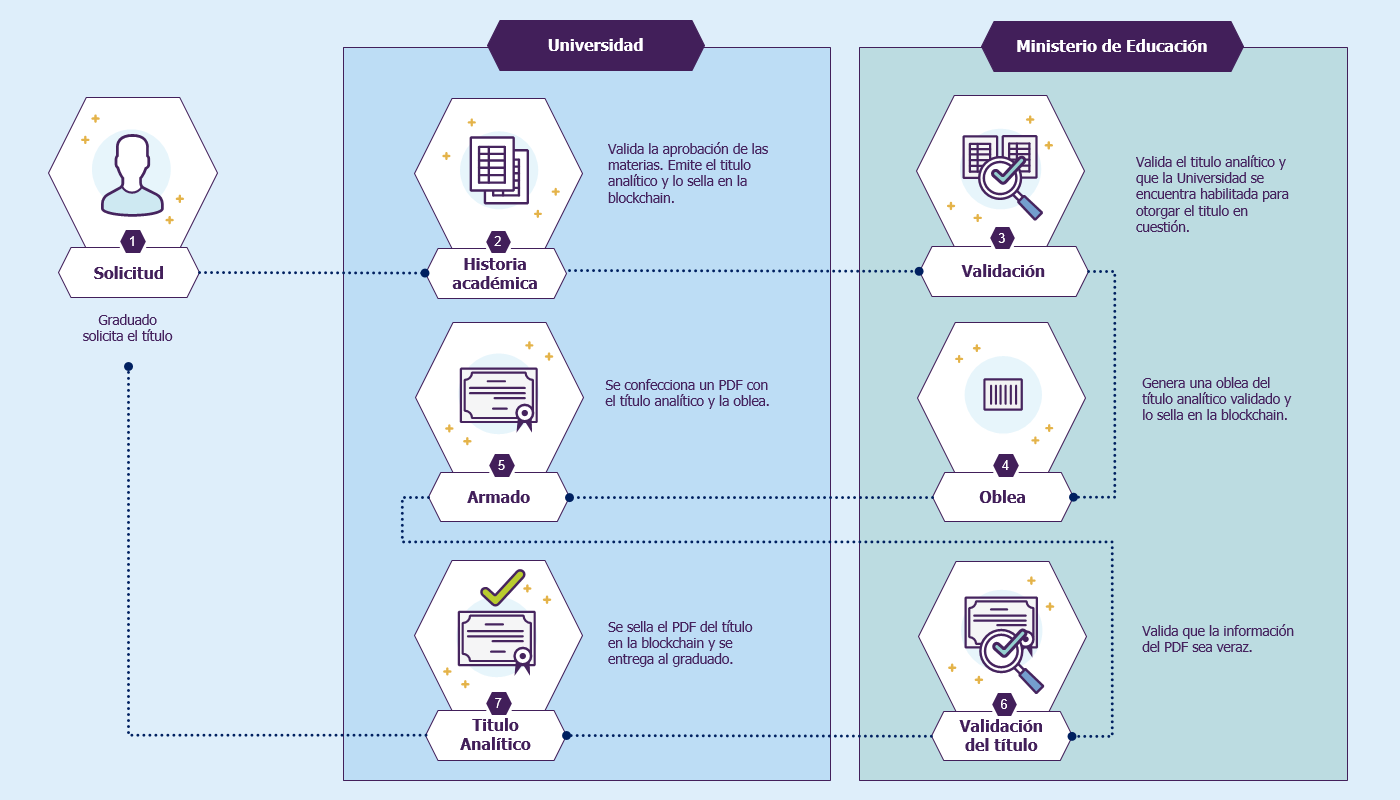
\includegraphics[width=\textwidth]{Img/cuadro_problematica.png}
            \caption{Petición del título.}
            \label{fig:cuadro_problematica}
        \end{figure}

        \subsection{Smart Degrees}
        
        Smart Degrees \cite{smart-degrees} es una plataforma que permite al usuario mediante una Dapp la registración y
        certificación de diplomas y títulos académicos. Esto lo hace basandose en la premisa de que el 
        exito en el mercado laboral, depende de la certificación de los títulos obtenidos.

        Para lograr su objetivo emplean la tecnología blockchain con la cual proporcionan y añade una mayor agilidad,
        comodidad y seguridad. Con lo cual permite gestionar y compartir el titulo universitario en plataformas de trabajo, 
        reclutadores y terceros.

        %cambios de lauti
        Hoy en dia esta aplicación es utilizada por muy pocas universidades, la gran mayoria son Españolas. 
        La aplicación permite subir la información del título de forma sencilla para su posterior validación, 
        lo que elimina una gran cantidad de intermediarios (Ver Figura \ref{fig:smart-degrees}).
        
        \begin{figure}
            \centering
            
\includegraphics[width=.3\textwidth]{Img/smart-degrees.jpeg}
            \caption{Verificación del título en \textbf{Smart Degrees}.}
            \label{fig:smart-degrees}
        \end{figure}


    \section{Objetivos}

        \subsection{Objetivo principal}

        Implementar las bases de un sistema en la blockchain que permita la generacion 
        y autenticacion de los titulos universitarios. 
        
        \subsection{Objetivos secundarios}

        \begin{itemize}
            \item Analizar los procesos que implican la generación y validación de un título.
            \item Evaluar el ecosistema de tecnologías a implementar.
            \item Diseñar los componentes de la aplicaciones.
            \item Implementar el sistema utilizando la BFA. 
        \end{itemize}


    \section{Desafíos}

        Esta sección tiene como objetivo describir los desafios que se deben afrontar para poder realizar la aplicación propuesta.

        \subsection{Modelo y procesos del negocio} 

            El primer desafio planteado implica analizar y comprender por parte del equipo, los procesos que implican la 
            generación y validación de un título universitario. Esto tiene como objetivo replicar y mejorar los procesos 
            en el sistema a construirse.
        
        \subsection{Aprendizaje de tecnologias} 

            El segundo desafio sera aprender las siguientes tecnologias:
            
            \begin{itemize}
                \item Blockchain Federal Argentina
                \item React
                \item NodeJS
            \end{itemize}
            
            Las tecnologías planteadas tienen como objetivo crear una arquitectura viable y limpia para el desarrollo del sistema.
            
            
        \subsection{Difusion del sistema} 

            Por ultimo se debe realizar una difusión del ecosistema planteado y lograr una aceptación por parte de los alumnos y las diferentes entidades.
            El objetivo de este desafio es lograr una mejora en la gestion de títulos, eliminando los intermediarios y facilitando la accesibilidad 
            a los documentos universitarios. 

    \section{Etapas}

        La forma de trabajo a llevar a cabo sera la siguiente:

        \begin{table}[H]
            \centering
            \begin{tabular}{|a|c|}
                \rowcolor{DayliGreen}
                \hline \mc{1}{Activdad} & \mc{1}{Tiempo estimado [meses]} \\ 
                \hline Prueba de concepto en la BFA & 4\\
                \hline Planificación de los smart contracts & 5\\
                \hline Analisis & 4\\
                \hline Diseño de la arquitectura & 6\\ 
                \hline Desarrollo de los smart contracts & 4\\
                \hline Desarrollo del backend & 10\\ 
                \hline Desarrollo del frontend & 10\\ 
                \hline Despliegue sobre BFA & 2\\
                \rowcolor{LightGreen}
                \hline \mc{1}{Tiempo total [años]}  & \mc{1}{3.75} \\
                \hline
            \end{tabular}
            \label{tab:etapas}
        \end{table}

        El tiempo establecido considera una dedicación no exclusiva al proyecto.
 
    \section{Conclusiones}

    Actualmente desarrollar aplicaciones sobre la blockchain agrega un nivel mas de complejidad debido
    a que es una tecnología es relativamente nueva. Esto hace que el desarrollador se convierta en un 
    curador de codigo, debido a que siempre que sale una nueva versión de las herramientas que se 
    utilizan para el desarrollo de las aplicaciones o Dapps, debe comprender los cambios y aplicarlos sobre el
    proyecto, esto desemboca en una mayor comprensión de las tecnologias.
    
    El desarrollo de la aplicación planteada en los puntos anteriores ahorraría mucho tiempo en la generación y 
    validación del título universitario. Pasando de tardar días o meses a tardar cuestion de minutos y generando confianza por parte de 
    la entidad que requiera su validación. Por otro parte esto significa un ahorro en papel, si bien esta implementación no esta 
    libre del consumo de energía es mucho menor al que se consume durante todo el circuito de emisión de un título.




\bibliographystyle{IEEEannot}
\bibliography{biblio}
\end{document}